\section{Implementations}\label{sec:implementation}
In this section, we describe the implementation details of the CloudCache framework. Specifically, we will use the 3-SAT problem as the sample to illustrate the infrastructure, software architecture, and programming interface.

\subsection{The CloudCache Infrastructure}
As is shown in Fig.~\ref{fig:system}, the infrastructure in the cloud consists of four different types of nodes: Master Node, Slave Node, Data Node and Sink Node. Outside of the cloud infrastructure, we have a Client which will submit the job to the Master Node. After the job is done, the Sink Node will push the job results to the Client.

The Master Node runs a multi-threaded TCP server, waiting for the job submitted from the Client. We consider the possibility of concurrent job submission from the clients, then the multi-threaded server is required. However, we do not optimize the server's performance under some pressure test. The Slave Node is also a multi-threaded TCP server, but once the Slave Node receives the job distributed from the Master Node, it will fork a worker thread to execute every task in the job. We do not fork multiple threads for each task because we do not want the first arrive job's tasks overwhelm the Slave Node (it is possible for Slave Node to run different jobs concurrently).

The Data Node is a tricky part in the system, because we combine the Slave Node and Data Node together in single physical machine. So a machine in the cloud will both solve the problem and host the data. We use hash function to shard the solution's cache choice. The reason for this implementation is that we want to maximize the possibility of local cache query and avoid unnecessary and frequent remote cache check which is very time consuming. In addition, we do not choose SQL database such as MySQL as the local storage system, but use some NoSQL techniques such as Redis~\cite{macedo2011redis} to be the persistent data storage. We believe the NoSQL techniques have much better performance to manage the key/value objects.

Finally, the Sink Node is the one to collect all the results and provide the final job result to the Client. To avoid the Slave Node's highly frequent task report, we buffer the report at the Slave Node until the buffer is full. This small optimization reduce the load of Sink Node, and increase the Slave Node's efficiency as well (task reporting blocks the Slave Node moving forward).

\begin{figure}
\centering
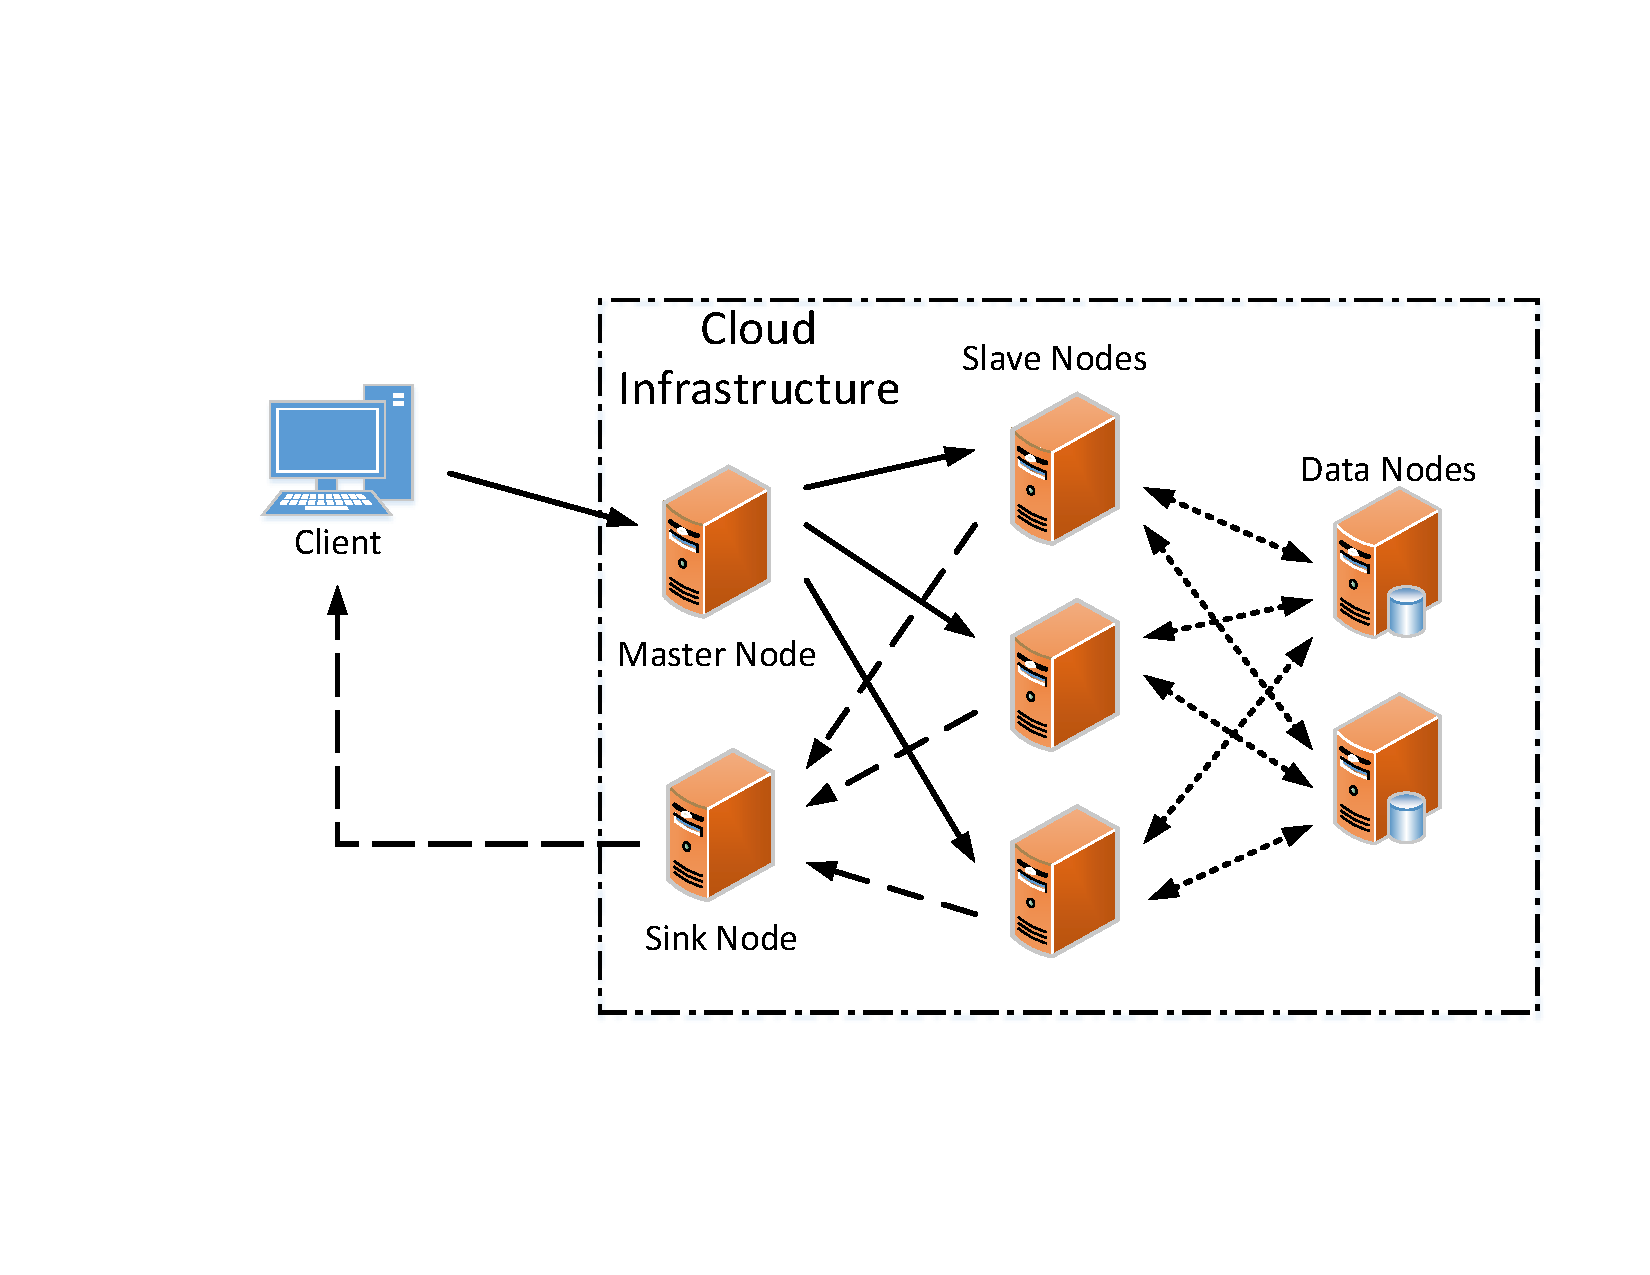
\includegraphics[width=0.5\textwidth]{pics/cloud-cache-arch.pdf}
\caption{The CloudCache System Diagram}
\label{fig:system}
\end{figure}

\subsection{Software Architecture}
We use Python as the language to implement the system. It consists of seven major modules in the source code.

\begin{itemize}
\item master.py. This module is the component to start a Master Node, which contains a multi-threaded TCP server, job class and some global variables for bookkeeping and statistics.

\item slave.py. This module is the component to start a Slave Node. It includes a multi-threaded TCP server as well, and a job execution handler and some statistic variables.
\item sink.py. The Sink Node module which receives the accumulated task report and dump the solutions to disk. After the job finished, the Client can come to retrieve the results.
\item kernel.py. The core module to kernel-solver. A developer should define a class to solve the problem, then the Slave Node will call the kernel-solver based on the configuration.
\item tools.py. It defines many helper class to help simplify the architecture like JobDispatcher, etc.
\item configure.py. The place is used to define any global configuration details, for instance, the Master Node, Slave Node, Data Node and Sink Node.
\end{itemize}

For the Redis server, it has to be deployed before running any module in the Data Node. Since we combine the Data Node and Slave Node into one physical machine, the Redis server is running as a service in the operating system.

\subsection{Programming Interface}
Two important programming interface in the CloudCache is in the tools.py module. The two APIs are \emph{tools.PersistentStorageManager.query(key)} and \emph{tools.PersistentStorageManager.push(key, value)}. 

A developer can call these two APIs to simply the cache operations in the implementation of kernel-solver. The kernel-solver is an abstract name, however, in practice, a developer needs to implement the solver class. For example, the 3-SAT problem, we implement \emph{BaseKernel3SAT} and \emph{CloudCacheKernel3SAT} classes which will be instantiated in job execution handler. Again, the developer does not need to pay additional attention to the data structure of key and value, because the two APIs above will serialize the key and value first before conducting cache operations.
